\documentclass[11pt,a4paper]{article}
\usepackage[T1]{fontenc}
\usepackage[margin=2.3cm]{geometry}
\usepackage{amsmath,amssymb}
\usepackage{graphicx}
\usepackage[dvipsnames]{xcolor}
\usepackage{enumitem}
\usepackage[colorlinks=true,linkcolor=blue,urlcolor=blue]{hyperref}
\setlength{\parskip}{0.6em}
\setlength{\parindent}{0pt}
\begin{document}

\begin{center}{\LARGE\bfseries openvectors}\\[0.4em]{\large Add forces and velocities as arrows and land a boat across a river, in three sessions.}\\[0.2em]\small PAN IIT OSS explainer \textbullet{} secondary school to diploma / undergraduate (levels 3-5)\end{center}

\section*{Why this exists}
Forces, velocities and displacements are all arrows. This explainer shows how to add them, split them into parts, take their dot product, and use them to steer a boat across a river, so you can build it yourself.

\section*{The end goal}
Add forces and velocities as arrows to land a boat across a river. The end goal is to land a boat across a river by adding the arrows of the boat, the current and the wind. The same arithmetic describes aircraft in a crosswind, forces on a structure and the work done by a force.

\section*{How the three sessions build up}
\begin{enumerate}[nosep]
\item \textbf{Session 1: Arrows that add up} (Level 1, conceptual interactive model, 60 min).
\item \textbf{Session 2: Components, trigonometry and the dot product} (Level 2, mathematical engineering model, 75 min).
\item \textbf{Session 3: A river that changes, and a boat that corrects itself} (Level 3, simulation and validation, 90 min).
\end{enumerate}

\section{Session 1: Arrows that add up}

\subsection*{A. Real-world problem}
You row a boat at 4 m/s straight at a landing on the far bank of a 60 m wide river. The river flows past at 2 m/s. You keep pointing at the landing, but the water keeps carrying you sideways. Where do you actually land? And how should you point the boat so that you land exactly opposite?

\subsection*{B. Concept and theory}
A velocity is an arrow: its length is the speed and its direction is where it points. We use x for downstream (along the river) and y for across the river, so an arrow is a pair (vx, vy). The boat's own arrow is what the boat would do in still water; the current's arrow is what the water does to everything in it. The boat's real motion over the ground is the sum of the two: put the tail of the second arrow on the head of the first and draw the arrow from the first tail to the last head. With numbers, add the matching entries. Because the across part of the ground arrow is what moves the boat to the far bank, the crossing time is the width divided by that part, and the sideways drift is the along-river part times that time.

\begin{itemize}[nosep]
\item v: boat speed through the water (m/s)
\item u: current speed (downstream) (m/s)
\item h: heading: angle from straight across, positive leaning upstream (degrees)
\item (gx, gy): ground arrow: along the river and across (m/s)
\item W: river width (60) (m)
\item T: crossing time (s)
\item drift: landing point along the river, positive downstream (m)
\end{itemize}

\begin{equation*}
\mathbf g=\mathbf b+\mathbf c,\qquad \mathbf b=v(-\sin h,\ \cos h),\quad \mathbf c=(u,\ 0)
\end{equation*}

\begin{equation*}
T=\frac{W}{g_y}=\frac{W}{v\cos h}
\end{equation*}

\begin{equation*}
\text{drift}=g_x\,T=\frac{(u-v\sin h)\,W}{v\cos h}
\end{equation*}

\begin{equation*}
\text{land opposite: } g_x=0\ \Rightarrow\ \sin h=\frac{u}{v}
\end{equation*}

\begin{center}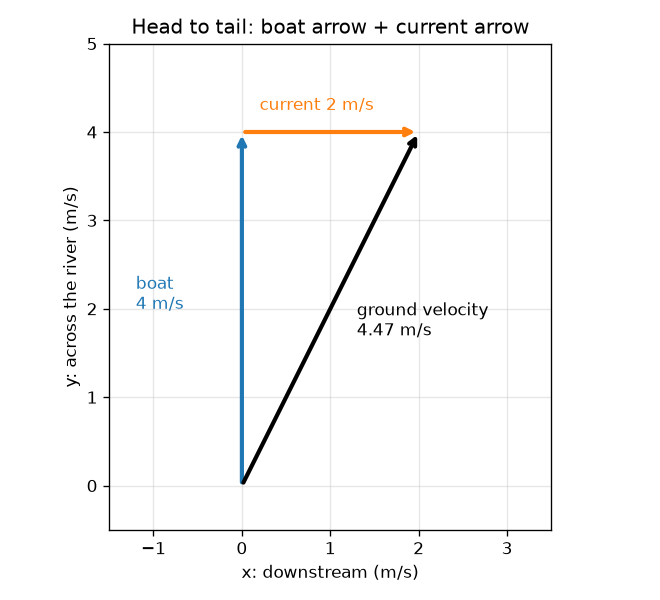
\includegraphics[width=0.85\linewidth]{figures/s01_head_to_tail.png}\\\small Head to tail: the boat arrow and the current arrow add up to the ground arrow.\end{center}

\subsection*{E. Worked example}
A boat of 4 m/s points straight across a 60 m river with a 2 m/s current. Find the ground arrow, the crossing time and the landing point. Then find the heading that lands the boat exactly opposite.
\begin{enumerate}[nosep]
\item Boat arrow = (0, 4) m/s (straight across, nothing along the river). Current arrow = (2, 0) m/s.
\item Ground arrow = (0 + 2, 4 + 0) = (2, 4) m/s. Its length is sqrt(2\textasciicircum{}2 + 4\textasciicircum{}2) = sqrt(20) = 4.47 m/s.
\item Only the across part moves the boat to the far bank: T = 60 / 4 = 15 s.
\item Drift = 2 m/s * 15 s = 30 m downstream.
\item To land opposite the along-river part must be zero: 2 - 4 sin h = 0, so sin h = 0.5 and h = 30 degrees upstream.
\item Then gy = 4 cos 30 = 3.46 m/s, so T = 60 / 3.46 = 17.3 s: the safer landing costs 2.3 s.
\end{enumerate}
\textbf{Answer.} Pointing straight across: ground arrow (2, 4) m/s, 15 s, landing 30 m downstream. Pointing 30 degrees upstream: ground arrow (0, 3.46) m/s, 17.3 s, landing exactly opposite.

\subsection*{F. Questions}
\begin{enumerate}[nosep]
\item \textbf{Conceptual.} Why must the boat point upstream to land exactly opposite its start? What does the sideways part of the boat arrow have to do?
\item \textbf{Numerical.} A boat of 5 m/s points straight across a 60 m river with a 3 m/s current. Find the crossing time, the landing point and the speed over the ground.
\item \textbf{Graph and simulation interpretation.} On the landing-point graph, for a 4 m/s boat and a 2 m/s current, where does the curve cross zero and what is the landing point at heading 0? What does the curve do for negative headings (leaning downstream)?
\item \textbf{Design and optimisation challenge.} Design: the pier is 15 m downstream of the point opposite the start. Choose a heading for the 4 m/s boat in the 2 m/s current so that it lands at the pier, and state how long the crossing takes.
\end{enumerate}

\section{Session 2: Components, trigonometry and the dot product}

\subsection*{A. Real-world problem}
A ferry with speed 4 m/s must cross a 60 m wide river with a 2 m/s current. The captain has two wishes: land exactly opposite the start, and cross as fast as possible. Do they ask for the same heading? What does each cost? And how much work does a steady side wind do on the way?

\subsection*{B. Concept and theory}
An arrow of length r at an angle phi from the +x axis has components (r cos phi, r sin phi); going back, r = sqrt(vx\textasciicircum{}2 + vy\textasciicircum{}2) and phi = atan2(vy, vx). Adding arrows adds components. The dot product a . b = ax bx + ay by also equals \textbar{}a\textbar{}\textbar{}b\textbar{} cos(angle between them): it is zero for perpendicular arrows, and (a . b) / \textbar{}b\textbar{} is the length of the shadow (projection) of a on b. The work of a constant force F over a displacement d is W = F . d: only the part of the force along the motion counts. For the ferry with heading h, the ground arrow has components gx = u - v sin h and gy = v cos h. Landing opposite needs gx = 0; crossing fast needs gy as large as possible, which is heading 0.

\begin{itemize}[nosep]
\item r, phi: length and angle of an arrow from the +x axis (units of the arrow, degrees)
\item (vx, vy): components of an arrow (same as the arrow)
\item a . b: dot product (product of the units)
\item F, d: force and displacement arrows (N, m)
\item W: work done by the force (J (joules))
\item v, u, h: boat speed, current, heading (upstream of straight across) (m/s, m/s, degrees)
\item T, drift: crossing time and landing point along the river (s, m)
\end{itemize}

\begin{equation*}
\mathbf v=(r\cos\varphi,\ r\sin\varphi),\qquad r=\sqrt{v_x^2+v_y^2},\quad \varphi=\operatorname{atan2}(v_y,v_x)
\end{equation*}

\begin{equation*}
\mathbf a\cdot\mathbf b=a_xb_x+a_yb_y=|\mathbf a||\mathbf b|\cos\theta,\qquad \text{projection}=\frac{\mathbf a\cdot\mathbf b}{|\mathbf b|}
\end{equation*}

\begin{equation*}
W=\mathbf F\cdot\mathbf d
\end{equation*}

\begin{equation*}
g_x=u-v\sin h,\quad g_y=v\cos h,\quad T=\frac{W_r}{v\cos h},\quad \text{drift}=g_xT\ \ (W_r=60\ \mathrm{m})
\end{equation*}

\begin{equation*}
\text{opposite: } h=\arcsin\frac{u}{v}\ (u<v);\qquad \text{fastest: } h=0
\end{equation*}

\begin{center}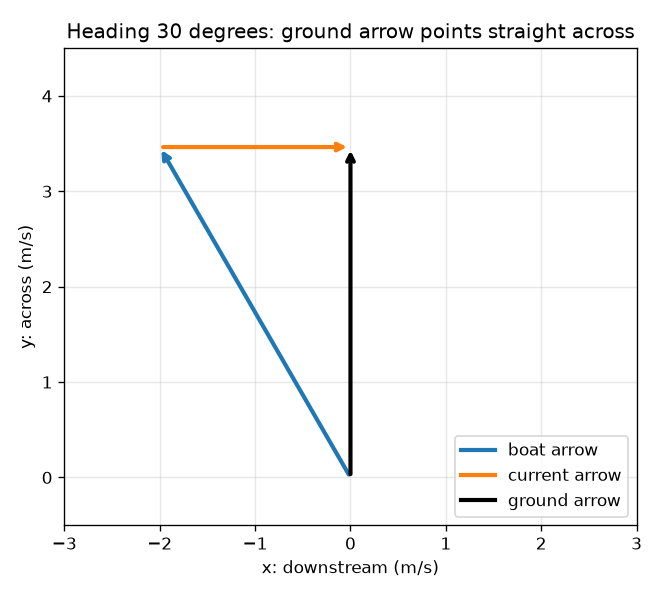
\includegraphics[width=0.85\linewidth]{figures/s02_components_30deg.png}\\\small At heading 30 degrees the ground arrow points straight across.\end{center}

\subsection*{E. Worked example}
Boat 4 m/s, current 2 m/s, river 60 m. Find (a) the heading that lands opposite, with its time; (b) the fastest crossing, with its landing point; (c) the work of a 20 N wind force pushing downstream while the boat goes straight across.
\begin{enumerate}[nosep]
\item (a) Opposite needs gx = 2 - 4 sin h = 0, so sin h = 0.5 and h = 30 degrees. gy = 4 cos 30 = 3.464 m/s, so T = 60 / 3.464 = 17.32 s.
\item (b) Fastest: gy = 4 cos h is largest at h = 0, gy = 4 m/s, T = 60 / 4 = 15 s. Drift = gx T = 2 * 15 = 30 m downstream.
\item (c) The displacement of the boat over the ground is d = (30, 60) m. The force is F = (20, 0) N.
\item W = F . d = 20 * 30 + 0 * 60 = 600 J. Only the along-river part of the displacement matters.
\item Check with the angle: \textbar{}d\textbar{} = sqrt(30\textasciicircum{}2 + 60\textasciicircum{}2) = 67.08 m, cos(angle) = 600 / (20 * 67.08) = 0.447, angle = 63.4 degrees; W = 20 * 67.08 * cos 63.4 = 600 J.
\end{enumerate}
\textbf{Answer.} (a) 30 degrees upstream, 17.32 s, landing opposite. (b) Straight across, 15 s, landing 30 m downstream. (c) 600 J.

\subsection*{F. Questions}
\begin{enumerate}[nosep]
\item \textbf{Conceptual.} Why is the fastest crossing always at heading 0, even when there is a current? Why does tilting upstream make the crossing slower?
\item \textbf{Numerical.} For a boat of 5 m/s and a current of 3 m/s on a 60 m river, find the heading that lands opposite, the crossing time, and the time and landing point of the fastest crossing.
\item \textbf{Graph and simulation interpretation.} From the crossing-time graph (v = 4, u = 2), what are the times at headings 0 and 30 degrees, and why does the curve rise slowly at first and then steeply?
\item \textbf{Design and optimisation challenge.} Design: the timetable allows at most 16 s for the 4 m/s ferry in the 2 m/s current, and the pier tolerates a landing within 5 m of the opposite point. Is there a heading that meets both? If not, which limit would you relax and by how much?
\end{enumerate}

\section{Session 3: A river that changes, and a boat that corrects itself}

\subsection*{A. Real-world problem}
Real rivers flow fastest in the middle and slowly near the banks, and the wind pushes the boat too. A fixed heading that works for a uniform current misses the landing. A ferry pilot watches where the boat is drifting and steers back towards the landing line. How can we simulate that, trust the simulation, and find out when no pilot could succeed? This is a simplified educational model, not a navigation tool.

\subsection*{B. Concept and theory}
We time-step the boat: at every small step dt we compute the boat's arrow, add the current's arrow at the boat's present position, and move the boat along the ground arrow. The current is parabolic: u(y) = 4 umax (y/W)(1 - y/W), zero at both banks and umax in mid-river, with an average of (2/3) umax. A side wind adds a constant w downstream. The naive pilot keeps one heading. The feedback pilot measures the cross-track error x (how far downstream of the target line the boat is) and sets heading = K x + Ki (sum of x dt), limited to +-60 degrees; K is in degrees per metre and Ki = K / 20. We solve the equations with the fourth-order Runge-Kutta method, and we validate against exact results: for a fixed heading the time is W / (v cos h) and the drift is (average current + wind - v sin h) times that time.

\begin{itemize}[nosep]
\item x, y: boat position: downstream and across the river (m)
\item v: boat speed through the water (m/s)
\item umax: peak current in mid-river (m/s)
\item w: side wind push, positive downstream (m/s)
\item theta: heading, positive leaning upstream (degrees)
\item K: feedback gain (degrees per metre)
\item dt: time step (0.05) (s)
\end{itemize}

\begin{equation*}
\dot x=u(y)+w-v\sin\theta,\qquad \dot y=v\cos\theta
\end{equation*}

\begin{equation*}
u(y)=4u_{\max}\frac{y}{W}\left(1-\frac{y}{W}\right),\qquad \bar u=\tfrac23u_{\max}
\end{equation*}

\begin{equation*}
\theta=\operatorname{clip}\!\Big(Kx+K_i\!\int x\,dt,\ \pm60^\circ\Big),\qquad K_i=K/20
\end{equation*}

\begin{equation*}
\text{fixed heading: } T=\frac{W}{v\cos\theta},\quad \text{drift}=(\bar u+w-v\sin\theta)\,T
\end{equation*}

\begin{equation*}
u>v\ (\text{uniform}):\quad \text{smallest drift}=\frac{W\sqrt{u^2-v^2}}{v}\ \text{at}\ \sin\theta=\frac vu
\end{equation*}

\begin{center}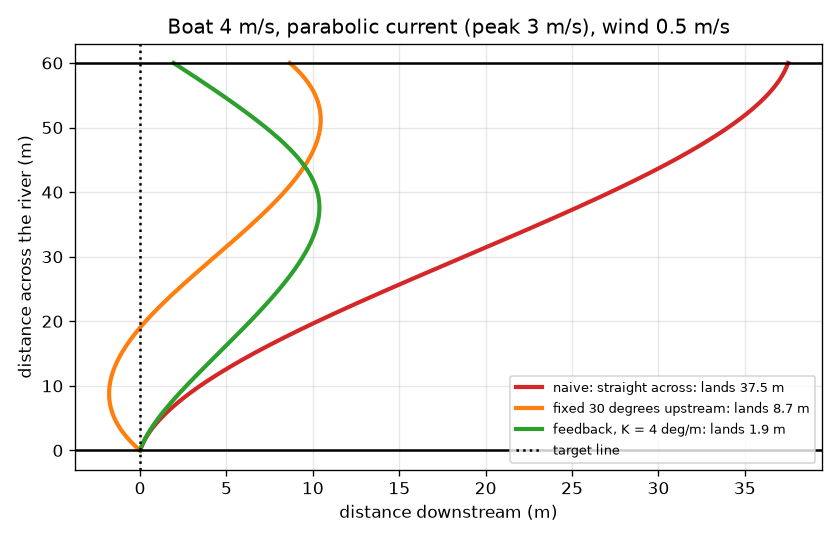
\includegraphics[width=0.85\linewidth]{figures/s03_paths_compared.png}\\\small Fixed heading (red), a tuned fixed 30 degree heading (orange) and feedback (green) on the same river.\end{center}

\subsection*{E. Worked example}
Boat 4 m/s, parabolic current with a 3 m/s peak, no wind, fixed heading straight across a 60 m river. Predict the drift and the time exactly, then compare with the simulation. Then add a 0.5 m/s wind.
\begin{enumerate}[nosep]
\item Time: T = 60 / 4 = 15 s for any current, because the across speed is 4 m/s.
\item The average current is (2/3) * 3 = 2 m/s, so the drift is 2 * 15 = 30 m. (This equals the integral of 4 * 3 (y/60)(1 - y/60) divided by the 4 m/s across speed.)
\item Simulation with dt = 0.05 s and Runge-Kutta: 30.000 m after 15.000 s.
\item With a 0.5 m/s wind the extra drift is 0.5 * 15 = 7.5 m, so the exact answer is 37.5 m, and the simulation gives 37.500 m.
\item Simulation versus the exact formula over 21 headings from -40 to 60 degrees: the largest difference is below 0.001 m, so the solver can be trusted here.
\end{enumerate}
\textbf{Answer.} Exact and simulated: 30.0 m drift in 15.0 s without wind, 37.5 m with a 0.5 m/s wind. The feedback boat in the same conditions (K = 4) lands 1.9 m downstream after 20.8 s.

\subsection*{F. Questions}
\begin{enumerate}[nosep]
\item \textbf{Conceptual.} Why does the feedback pilot use an integral term (the running sum of the error) as well as the proportional term K x?
\item \textbf{Numerical.} Using the exact formula, find the drift of a 4 m/s boat that points straight across a 60 m river with a parabolic current of peak 5 m/s and no wind. Check it against the sensitivity graph.
\item \textbf{Graph and simulation interpretation.} In the sensitivity graph, what is the feedback landing point for peak currents of 3, 5 and 6 m/s, and why does it get worse above 4 m/s?
\item \textbf{Design and optimisation challenge.} Design: for the 4 m/s boat, the parabolic current with a 3 m/s peak and a 0.5 m/s wind, choose the gain K (in steps of 0.5) so that the landing is within 2 m and the crossing takes at most 21 s. Justify your choice.
\end{enumerate}

\section{Real-world mini-project}
\textbf{Plan a ferry route.} A ferry with speed 4 m/s crosses a 60 m river with a 0.5 m/s side wind. The current is parabolic, with a peak of 2, 3 or 4 m/s depending on the season. The harbour wants the ferry to land within 2 m of the opposite pier and to cross in at most 23 s. Use \texttt{simulate} from Session 3 and scan the feedback gain K from 0.5 to 8 in steps of 0.5 for each peak current.

\section{The path ahead}
\begin{enumerate}[nosep]
\item \textbf{Session 4: A look-ahead heading controller.} A controller that, each step, picks the heading for which holding it to the far bank would land on the target line.
\item \textbf{Session 5: A pilot that does not know the wind.} A wind estimator built from the difference between the measured ground arrow and the arrow the model predicts.
\item \textbf{Session 6: Follow a river bend.} A simulation where the current follows a 90 degree bend of radius 150 m and the target line is the centre line.
\item \textbf{Session 7: Force systems: a tug and a barge.} A two-tug model where each tug pulls with a force arrow and the barge follows the resultant.
\item \textbf{Session 8: Animate the crossing with arrows.} A GIF of the crossing with the boat, current and ground arrows drawn on the boat.
\end{enumerate}

\section{Answers and hints}

\subsection*{Session 1}
\begin{enumerate}[nosep]
\item \textbf{Conceptual.} Hint: Landing opposite means the along-river part of the ground arrow is zero. Solution: The ground arrow is the boat arrow plus the current arrow. The current arrow points downstream, so to make the along-river part of the sum zero the boat arrow must have an equal and opposite upstream part. That is only possible by leaning the boat upstream. The across part of the boat arrow is then a little shorter than the full boat speed, so the crossing takes longer.
\item \textbf{Numerical.} Hint: Ground arrow = (3, 5). Time = width / across part. Solution: Ground arrow = (3, 5) m/s. T = 60 / 5 = 12 s. Drift = 3 * 12 = 36 m downstream. Speed over the ground = sqrt(3\textasciicircum{}2 + 5\textasciicircum{}2) = sqrt(34) = 5.83 m/s. Sanity check: faster than the boat alone (5 m/s) because the current helps along the river, and the 12 s is the time for 60 m at 5 m/s.
\item \textbf{Graph and simulation interpretation.} Hint: Read the curve at heading 0 and where it meets the horizontal line at 0. Solution: At heading 0 the curve is at 30 m. It crosses zero at heading 30 degrees. For negative headings, where the boat leans downstream with the current, the landing point is larger: the boat drifts even further downstream.
\item \textbf{Design and optimisation challenge.} Hint: Try headings in the app until the landing point reads 15 m, or compute the landing point for several headings with \texttt{crossing} from the lesson. Solution: A heading of about 15 degrees upstream gives a landing 15.0 m downstream (14.98 m for exactly 15 degrees) and a crossing time of about 15.5 s. Assumption: constant current and boat speed. Check: heading 0 gives 30 m and heading 30 gives 0 m, so a heading half way between lands about half way, near 15 m, because the curve is almost straight there.
\end{enumerate}

\subsection*{Session 2}
\begin{enumerate}[nosep]
\item \textbf{Conceptual.} Hint: Which component of the ground arrow carries the boat to the far bank? Solution: Only gy = v cos h carries the boat across, and the current has no across part. cos h is largest (1) at h = 0, so gy is largest and T = W / gy is smallest. Tilting trades some of the across speed for an upstream speed, so it cannot be faster; it is done only to cancel drift.
\item \textbf{Numerical.} Hint: sin h = u / v. Use the 3-4-5 triangle. Solution: sin h = 3/5 = 0.6, so h = 36.87 degrees. gy = 5 cos 36.87 = 4 m/s, T = 60 / 4 = 15 s. Fastest: h = 0, T = 60 / 5 = 12 s, drift = 3 * 12 = 36 m downstream. So the safe landing costs 3 s.
\item \textbf{Graph and simulation interpretation.} Hint: T = 60 / (4 cos h), and cos is flat near 0. Solution: T = 15 s at 0 degrees and 17.3 s at 30 degrees. Near h = 0 the cosine barely changes, so T hardly changes; at larger angles cos h falls quickly, so T rises steeply (at 60 degrees T = 30 s).
\item \textbf{Design and optimisation challenge.} Hint: Time at most 16 s gives cos h \textgreater{}= 60 / (4 * 16). Then check the landing point at the largest allowed heading. Solution: At most 16 s needs cos h \textgreater{}= 0.9375, so h \textless{}= 20.4 degrees; at that heading the landing point is still 9.7 m downstream, so no heading gives both limits. Options: accept a landing within 10 m (headings 20.1 to 20.4 degrees work) or allow 17 s (headings from 25.1 to 28.1 degrees land within 5 m). The trade-off is time against accuracy; the pier decides.
\end{enumerate}

\subsection*{Session 3}
\begin{enumerate}[nosep]
\item \textbf{Conceptual.} Hint: What heading does the boat need to hold in a steady wind, and what error does a purely proportional rule need in order to produce that heading? Solution: In a steady current and wind the boat needs a steady upstream heading just to stay on the line. A purely proportional rule produces a heading only when there is an error (heading = K x), so it must settle with a leftover error. The integral term keeps growing while the error persists and supplies the steady heading without a leftover error. Too much of it makes the boat overshoot the line.
\item \textbf{Numerical.} Hint: Drift = (2/3) umax * W / v for heading 0. Solution: Average current = (2/3) * 5 = 3.33 m/s; T = 15 s; drift = 3.33 * 15 = 50 m. This matches the red line of the sensitivity graph (10 m for each m/s of peak current: 5 * 10 = 50 m).
\item \textbf{Graph and simulation interpretation.} Hint: Read the green curve; think about the heading limit and the current plus the boat speed in mid-river. Solution: About 2.0 m at 3 m/s, 13.7 m at 5 m/s and 30.4 m at 6 m/s (the fixed heading gives 30, 50 and 60 m). Above 4 m/s the current in mid-river is faster than the boat, so no heading can hold the boat on the line there, and the heading is capped at 60 degrees; the boat is swept downstream in the middle and cannot fully return.
\item \textbf{Design and optimisation challenge.} Hint: Run \texttt{simulate(4, 3, 0.5, K=...)} for K = 3.5, 4, 4.5 and 5 and compare the landing point and the time. Solution: K = 3.5 lands 3.2 m off (too far). K = 4 lands 1.9 m off in 20.8 s: it meets both limits. K = 4.5 lands 1.0 m off but takes 21.2 s, over the limit; K = 5 lands 0.4 m off in 21.6 s. So K = 4 is the only half-step gain that satisfies both. Trade-off: a larger gain lands closer to the target but swings the heading upstream harder, so the crossing takes longer.
\end{enumerate}

\section{How to join}
Read \texttt{CONTRIBUTING.md} in the repository, then pick an issue labelled \texttt{good first issue}. Repository: \url{https://github.com/KrunalPanchal1995/openvectors}

\end{document}
